\documentclass[10pt, aspectratio=169]{beamer}

\usetheme{metropolis}
\metroset{block=fill}
\usepackage{appendixnumberbeamer}

\usepackage{booktabs}
\usepackage[scale=2]{ccicons}


\usepackage{siunitx}

\usepackage{xspace}
\newcommand{\themename}{\textbf{\textsc{metropolis}}\xspace}

\usepackage{amsmath}
\def\RR{\mathbb{R}}
\def\Pr{\mathrm{Pr}}

\usepackage{tikz}
\usetikzlibrary{positioning, arrows}
\usetikzlibrary{decorations.pathreplacing}
\usetikzlibrary{calc}
\usepackage{pgfplots}
\usepgfplotslibrary{dateplot}
\tikzset{
  font=\small,
  node distance=0.5cm and 0.2cm,
  bdata/.style={draw, rectangle, text width=2.2cm, align=center},
  sdata/.style={draw, rectangle, text width=1.75cm, align=center},
  bmodel/.style={rectangle, fill=mLightBrown, text width=4cm, align=center, rounded corners},
  smodel/.style={rectangle, fill=mLightBrown, text width=2.2cm, align=center, rounded corners},
  pred/.style={draw, rectangle, text width=1cm, align=center}
}

\usepackage[style=numeric]{biblatex}
\addbibresource{lit.bib}

\usepackage{xcolor}
\usepackage{hyperref}

\definecolor{mDarkTeal}{HTML}{23373b}
\definecolor{mLightBrown}{HTML}{EB811B}
\definecolor{mDarkBrown}{HTML}{B85002}
\definecolor{mLightGreen}{HTML}{14B03D}

\title{Beating the International Prognostic Index for high-risk DLBCL patients}
\subtitle{Master thesis progress report}
\date{March 12, 2024}
\author{Lukas Geßl}
\institute{Chair of Statistical Bioinformatics, Regensburg University}
% \titlegraphic{\hfill
\includegraphics[height=1.5cm]{logo.pdf}}

\begin{document}

\maketitle

% \begin{frame}{Table of contents}
%   \setbeamertemplate{section in toc}[sections numbered]
%   \tableofcontents[hideallsubsections]
% \end{frame}

\section{Setting the arena}

\begin{frame}{DLBCL: a heterogeneous cancer with a homogeneous therapy}

  Diffuse large B-cell lymphoma (DLBCL) is the most common type of B-cell lymphoma, 
  accounting for 30\% of all diagnoses.

  While DCBCL is a clinically very heterogeneous disease, there is only one treatment 
  regimen: immunochemotherapy with R-CHOP. It cures two thirds of the patients.

  Cure rates among relapsed or refractory patients are low, hence we should not send 
  them through the standard therapy in the first place, but into alternative, more 
  experimental treatments and trials instead. 
  
  We define relapsed or refractory patients or \alert{high-risk} patients as those with a 
  \alert{progression-free survival (PFS) < 2 years}.

\end{frame}

\begin{frame}{The goal of this thesis and the MMML-Predict project is ...}

  ... to develop a \alert{cost-efficent classifier filtering out high-risk DLBCL patients} before an R-CHOP 
  treatment begins or at least at an early stage of it. 

  Candidate input features are 

  \begin{itemize}
    \item clinical data (like the IPI, see next slide),
    \item transcriptomic (RNA-seq, signatures like LAMIS, ABC vs. GCB),
    \item proteomic signatures,
    \item somatic genetic factors (translocations like MYC),
  \end{itemize}

  all of which are measured \alert{at diagnosis}, as well \alert{dynamic} features like 

  \begin{itemize}
    \item imaging (PET-CT) after 2 cycles of R-CHOP,
    \item the tumor burden in the body determined via circulating tumor DNA (ctDNA) in a 
    liquid biopsy after 2 and 4 cycles of R-CHOP. 
  \end{itemize}

\end{frame}

\begin{frame}{To beat: the Internatinal Prognostic Index (IPI) for non-Hodgkin's lymphoma}

  The IPI \autocite{ipi93} is a simple risk score ranging from 0 to 5 depending on how many of the following 
  \alert{clinical} questions for a patient one can answer with "yes": 

  \begin{itemize}
    \item Age > 60?
    \item Ann Arbor stage III or IV: is the cancer advanced?
    \item Serum LDH (lactacte dehydrogenease) level: higher than normal?
    \item Performance status: is the patient no longer ambulatory? 
    \item Number of extranodal sites (like bone marrow, liver, lung) involved: more than one?
  \end{itemize}

  The lower the IPI, the better the patient's outlook: higher progression-free survival (PFS) and 
  overall survival (OS).

\end{frame}

\begin{frame}{The IPI is a 30-year old dinosaur}

  Yet, it's still state of the art in clinical practice when it comes to assessing a DLBCL 
  patient's risk even in the age of multi-omics because it's \alert{simple}, \alert{cheap} and 
  \alert{robust} (after all, it's based on a rigorous statistical analysis and Cox regression).

  Still, just six values the IPI can attain mean it's very rough. In particular, it fails 
  to identify a clinically relevant high-risk group:

  \begin{itemize}
    \item The cohort with IPI $\leq 5$ is \alert{too small} to significantly differ from the rest in terms 
    of survival and to get attention from clincians.
    \item The cohort with IPI $\leq 4$ \alert{lacks precision in identifying high-risk patients}: 16\% of
    patients have an IPI $\leq 4$, but only 40\% of them are high-risk. This is too low to persuade 
    a clinician to change the treatment plan.
  \end{itemize}

\end{frame}

\begin{frame}{What does "beating the IPI" mean?}

  We need \alert{data} to demonstrate the new classifier on. The MMML-Predict project is enrolling 200 DLBCL 
  patients in a training cohort right now, 100 will follow for the validation cohort. For my thesis,
  I need to use already existent data.

  Being better than the IPI means, on the validation cohort the new classifier needs to 

  \begin{itemize}
    \item be \alert{more precise in identifying high-risk patients} than the IPI: the 95\% confidence interval (CI) 
    of the precision (proportion of true positives among all positives; according to Clopper-Pearson) must 
    not include 35\%, the precision of IPI $\geq 4$ on pooled data from DSNHNL trials ($\num{2721}$ samples),
    \item yield \alert{two cohorts with significantly differing survival} (PFS): logrank test p-value < 0.05.
  \end{itemize}

  Calculations with the size of the validation cohort ($n = 100$) suggest that a precision $\geq 50\%$ is enough.
\end{frame}

\section{Meet the players}

\begin{frame}{\alert{Early} versus late integration}
  \begin{columns}
    \column{0.5\textwidth}
      \centering
      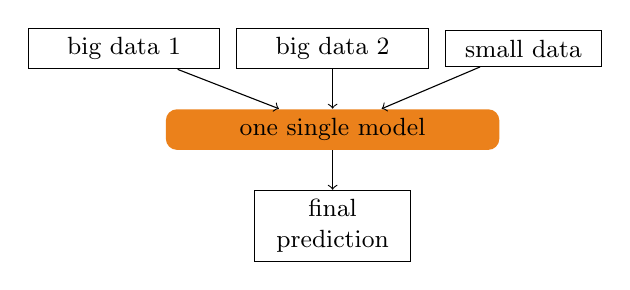
\begin{tikzpicture}
        \node[bdata] (bigdata1) {big data 1};
        \node[bdata, right=of bigdata1] (bigdata2) {big data 2};
        \node[sdata, right=of bigdata2] (smalldata) {small data};
        \node[bmodel, below=of bigdata2] (latemodel) {one single model};
        \node[sdata, below=of latemodel] (latepred) {final prediction};
        
        \draw[->] (bigdata1) -- (latemodel);
        \draw[->] (bigdata2) -- (latemodel);
        \draw[->] (smalldata) -- (latemodel);
        \draw[->] (latemodel) -- (latepred);
      \end{tikzpicture}
    \column{0.5\textwidth}
      \begin{itemize}
        \item Provide all data as input features to a single model.
        \item Upside: easy to implement, one algorithm fits and picks the model 
          including cross validation.
        \item Downside: data on vastly different scales may confuse the model and 
          its minimizer.
      \end{itemize}
  \end{columns}
\end{frame}

\begin{frame}{Early versus \alert{late} integration}
  \begin{columns}
    \column{0.5\textwidth}
      \centering
      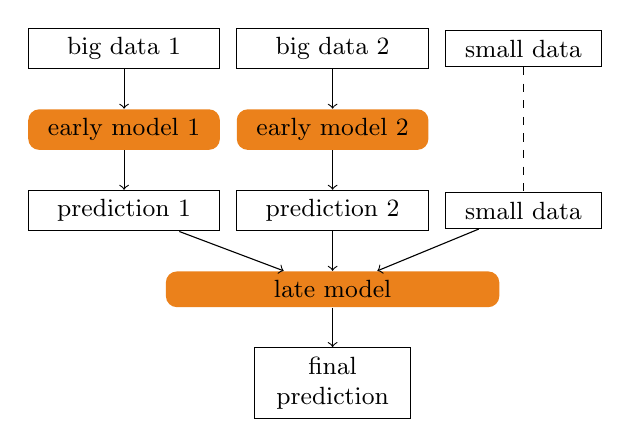
\begin{tikzpicture}  
        \node[bdata] (bigdata1) {big data 1};
        \node[bdata, right=of bigdata1] (bigdata2) {big data 2};
        \node[sdata, right=of bigdata2] (smalldata) {small data};
        \node[smodel, below=of bigdata1] (earlymodel1) {early model 1};
        \node[smodel, right=of earlymodel1] (earlymodel2) {early model 2};
        \node[bdata, below=of earlymodel1] (earlypred1) {prediction 1};
        \node[bdata, right=of earlypred1] (earlypred2) {prediction 2};
        \node[sdata, right=of earlypred2] (esmalldata) {small data};
        \node[bmodel, below=of earlypred2] (latemodel) {late model};
        \node[sdata, below=of latemodel] (latepred) {final prediction};
        
        \draw[->] (bigdata1) -- (earlymodel1);
        \draw[->] (earlymodel1) -- (earlypred1);
        \draw[->] (bigdata2) -- (earlymodel2);
        \draw[->] (earlymodel2) -- (earlypred2);
        \draw[dashed] (smalldata) -- (esmalldata);
        \draw[->] (earlypred1) -- (latemodel);
        \draw[->] (earlypred2) -- (latemodel);
        \draw[->] (esmalldata) -- (latemodel);
        \draw[->] (latemodel) -- (latepred);
      \end{tikzpicture}
    \column{0.5\textwidth}
      \begin{itemize}
        \item Early models deal with high-throughput data and its problems: overfitting, 
          systematic errors.
        \item Upside: modularizes the model selection process, allows for very
          sophisticated late models.
        \item Downside: implementing the model selection process becomes more 
          complicated, how to deal with cross validation in the early models?
      \end{itemize}
  \end{columns}
\end{frame}

\begin{frame}{The key player for early-stage models: the zeroSum package}
  We feed high-troughput data into 

  \begin{itemize}
    \item \alert{Cox} proportional-hazards models and
    \item \alert{logistic} models,
  \end{itemize}

  both endowed with \alert{LASSO} regularization and the \alert{zero-sum} constraint. More precisely, we 
  aim to estimate the response $y_i$ of sample $i$ by a predictor $x_i \in \mathbb{R}^p$ via 
  \begin{align}
    y_i = f(\beta_0 + x_i^T \beta) + \varepsilon_i
  \end{align}
  for a link function $f: \mathbb{R} \to \mathbb{R}$, a set of coefficients $(\beta_0, 
  \beta)$, and a residual $\varepsilon_i$.
\end{frame}

\begin{frame}{The zero-sum constraint}
  We demand $\sum_{j=1}^p \beta_j = 0$, the zero-sum constraint. Why?

  \begin{itemize}
    \item Keep in mind: $x_i$ is usually the result of taking the logarithm of original 
      observations $x_i'$, i.e. $x_{ij} = \log(x_{ij}')$ for all $j$.
    \item If we rescale $x_i'$ by a factor $\gamma > 0$, then $x_i$ changes by an additive 
      constant, $\log(\gamma)$: $\log(\gamma x_{ij}') = \log(\gamma) + \log(x_{ij}')$ for all j.
    \item The zero-sum consraint ensures $\sum_{j=1}^p \beta_j (\log(\gamma) + \log(x_{ij}')) = 
      \sum_{j=1}^p \beta_j \log(\gamma) + \sum_{j=1}^p \beta_j x_{ij} = 0 + \sum_{j=1}^p 
      \beta_j x_i$. 
  \end{itemize}
  
  In particular, $f(\beta_0 + \log(\gamma x_i')^T \beta) = f(\beta_0 + \log(x_i')^T \beta)$: the 
  model is \alert{invariant under rescaling}.

  This comes at a price: model training takes more computation time.
\end{frame}

\begin{frame}{Wrap it all into a loss function}
  Training such a models comes down to minimizing a loss function of the form 
  \begin{align}
    \mathcal{L}_{X, y, \lambda, v, w}(\beta_0, \beta) = -\sum_{i=1}^n w_i 
    \ell(\tilde{y}_i, \beta_0 + x_i^T \beta) + \lambda \sum_{j=1}^p v_j |\beta_j| 
    \quad \text{subject to } \sum_{j=1}^p u_j \beta_j = 0
  \end{align}
  for hyperparameters 
  \begin{itemize}
    \item $\lambda > 0$, the LASSO penalty factor (tuned in a cross-validation),
    \item $u \in \RR^p$, the zero-sum weights (often $u = \mathbf{1}$),
    \item $v \in \RR^p_{\geq 0}$, the LASSO penalty weights (often $v = \mathbf{1}$), and
    \item $w \in \RR^n_{\geq 0}$, the sample weights (often $w = \frac{1}{N} \mathbf{1}$).
  \end{itemize}

  $\ell: \RR^2 \to \RR$ is a model-dependent log likelihood. $\tilde{y}_i$ is closely 
  related to $y_i$ (if not the same), its nature again depends on the model.
\end{frame}

\begin{frame}{Lifting the curtain on $\ell$ and $y_i$ for the \alert{Cox} model}
  $y_i$ is the \alert{relative hazard} of sample $i$: the higher it is, the earlier we 
  expect sample $i$ to face the event (cancer progression in our case) compared to the 
  other samples.

  $\tilde{y}_i$ is the time to event.

  $\ell$ tries to enforce the correct ordering: $\beta_0 + x_i^T \beta$ should be monotonic 
  in $\tilde{y}_i$.

  \begin{alertblock}{Practical remark}
    Patients often drop out of a study before the event occurs (so-called right censoring).
    The Cox model can make use of the information that a sample was event-free for at least 
    a certain amount of time, so we needn't discard right-censored samples.
  \end{alertblock}
\end{frame}

\begin{frame}{Lifting the curtain on $\ell$ and $y_i$ for the \alert{logistic} model}
  We need to \alert{threshold the time to event} to get a \alert{binary response}: 
  $\tilde{y}_i = y_i = 1$ if the event happens before a certain time $T$, $0$ otherwise. 
  The most straightforward choice is $T = 2$ years in our case. But: one can view \alert{$T$} 
  as yet \alert{another hyperparameter}.
  
  We want to write 
  \begin{align}
    p(x_i) = \Pr(y_i=1 | x_i) = \frac{1}{1 + \exp(-(\beta_0 + x_i^T \beta))}
  \end{align}
  and try to enforce this with 
  \begin{align}
    \ell(y_i, \beta_0 + x_i^T \beta) = y_i \log p(x_i) + (1 - y_i) \log(1 - p(x_i)).
  \end{align}

  \begin{alertblock}{Practical remark}
    When binarizing the data, we need to discard samples right-censored before $T$.
  \end{alertblock}
\end{frame}

\section{Train the players and select the best}

\begin{frame}{Train-test paradigm}
  \begin{columns}
    \column{.5\textwidth}
      \centering
      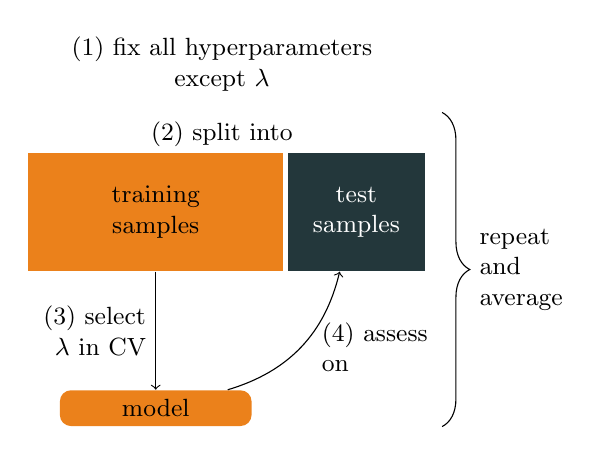
\begin{tikzpicture}[
        node distance=1cm and 0.05cm,
        trainn/.style={rectangle, text width=3cm, align=center, fill=mLightBrown, minimum height=1.5cm},
        testn/.style={rectangle, text width=1.5cm, align=center, fill=mDarkTeal, text=white, minimum height=1.5cm},  
        fixn/.style={rectangle, text width=4.7cm, align=center},
        splitn/.style={rectangle, text width=4.5cm, align=center}
        ]
        \node[trainn] (traindata) {training\\ samples};
        \node[testn, right=of traindata] (testdata) {test samples};
        \node[splitn, above=0.7cm of $(traindata)!0.33!(testdata)$] (split) {(2) split into};
        \node[fixn, above=0.15cm of split] (fixhyper) {(1) fix all hyperparameters\\ except $\lambda$};
        \node[smodel, below=1.5cm of traindata] (model) {model};
        
        \draw[->] (traindata) -- node[midway, left, align=right] {(3) select\\ $\lambda$ in CV} (model);
        \draw[->] (model) to[bend right] node[midway, right=4pt, align=left] {(4) assess\\ on} (testdata);

        \path let \p1 = (split.east) in \pgfextra{\xdef\bracex{\x1}};
        \path let \p1 = (split.north) in \pgfextra{\xdef\braceuy{\y1}};
        \path let \p1 = (model.south) in \pgfextra{\xdef\bracely{\y1}};
        \draw[decorate,decoration={brace,amplitude=10pt,mirror,raise=12pt}] 
          (\bracex, \bracely) -- (\bracex, \braceuy) node[midway, right=22pt, align=left] {repeat\\ and\\ average};
      \end{tikzpicture}
    \column{.5\textwidth}
      \alert{Hyperparameters} excluding $\lambda$ may be
      \begin{itemize}
        \item the model type,
        \item zero-sum weights, regularization weights, sample weights,
        \item the threshold $T$ for the logistic model\footnotemark{}.
      \end{itemize}
      We \alert{assess} the models
      \begin{itemize}
        \item with a scalar metric (like the ROC-AUC) to get a \alert{pre-selection},
        \item in scatter plots (like prevalence versus precision) to \alert{threshold the scores} 
          output by the pre-selected models.
      \end{itemize}
    \end{columns}
    \footnotetext{Similarly for the Cox model, we can right-censor samples with time to event $> T$ at $T$.}
\end{frame}

\begin{frame}{Software}
  To fit and cross-validate the logistic and Cox models I rely on the \alert{zeroSum R package} 
  by Thorsten Rehberg \autocite{zerosumR}. It extends the glmnet package by the zero-sum constraint.

  When integrating a model found in a cross validation into another model I want to continue the cross 
  validation of the early model. zeroSum does not report enough details, so I added this functionality in 
  a \alert{fork zeroSumLI} \autocite{zerosumliR}.

  Training and assessing a bunch of models on several data sets means a lot of administrative, repetitive 
  work. I automized and outsourced this part into an \alert{R package lymphomaSurvivalPipeline} \autocite{lspR}.
\end{frame}

\section{Watch the game}

\begin{frame}{The data}
  I trained models predicting progression-free survival $< 2$ years on data including bulk RNA-seq 
  taken from Schmitz et al. \autocite{schmitz18}. 
  \begin{columns}
    \column{.6\textwidth}
      \begin{itemize}
        \item It has $n = \num{229}$ patients with survival information, $p = \num{25066}$ genes.
        \item $\num{78}$ (34\%) of these are high risk.
        \item $\num{135}$ (59\%) are low risk. 
        \item $\num{16}$ (7\%) we cannot assign.
        \item All IPI features are available in pheno data.
        \item The IPI does a pretty good job on it, see Table \ref{fig:ipi-schmitz}.
      \end{itemize}
    \column{.4\textwidth}
      % latex table generated in R 4.3.2 by xtable 1.8-4 package
% Mon Feb 19 15:25:19 2024
\begin{table}[ht]
\centering
\begin{tabular}{rrr}
  \hline
IPI $\geq$ & prevalence & precision \\ 
  \hline
  5 & 0.01 & 1.00 \\ 
    4 & 0.13 & 0.65 \\ 
    3 & 0.35 & 0.55 \\ 
    2 & 0.59 & 0.48 \\ 
    1 & 0.85 & 0.41 \\ 
    0 & 1.00 & 0.37 \\ 
   \hline
\end{tabular}
\caption{Classifying PFS < 2 years on \autocite{schmitz18}.} 
\label{fig:ipi-schmitz}
\end{table}

    \end{columns}
\end{frame}

\begin{frame}{The results}
  \small
  % latex table generated in R 4.3.2 by xtable 1.8-4 package
% Mon Feb 19 15:25:19 2024
\begin{table}[ht]
\centering
\begin{tabular}{rlrr}
  \hline
rank & model & $T$ & AUC \\ 
  \hline
   1 & logistic & 1.75 & 0.770 \\ 
     2 & logistic zerosum & 1.75 & 0.769 \\ 
     3 & cox & 1.75 & 0.762 \\ 
     4 & cox zerosum & 1.75 & 0.761 \\ 
     5 & cox & 2 & 0.755 \\ 
     6 & logistic zerosum & 1.5 & 0.755 \\ 
     7 & cox zerosum & 1.5 & 0.752 \\ 
     8 & cox & 1.5 & 0.750 \\ 
     9 & cox & Inf & 0.749 \\ 
    10 & cox zerosum & Inf & 0.748 \\ 
   \hline
\end{tabular}
\caption{Split into train and test cohort, train a model on train cohort, calculate ROC-AUC
        on test cohort. Repeat this 15 times and average.} 
\label{fig:top-auc-schmitz}
\end{table}

\end{frame}

\begin{frame}[standout]
  Thank you for your attention! \par Questions?
\end{frame}

\appendix

\begin{frame}[allowframebreaks]{References}
  \printbibliography
\end{frame}

\end{document}